%%%%%%%%%%%%%%%%%%%%%%%%%%%%%%%%%%%%%%
% This is the name of the style file.
%%%%%%%%%%%%%%%%%%%%%%%%%%%%%%%%%%%%%%
%
% phd  -> for a PhD dissertation
% ms   -> for an MS thesis
% If both phd and ms are used then phd will overide.  If none are used,
% then ms will be active by default.
%
% cpyr -> generate a copyright page
% lof  -> generate List of Figures
% lot  -> generate List of Tables
%\documentclass[ms,cpyr,lof,lot]{uathesis}
\documentclass[ms,cpyr]{uathesis}
%
%%%%%%%%%%%%%%%%%%%%%%%%%%%%%%%%
% List of any packages you use.
%%%%%%%%%%%%%%%%%%%%%%%%%%%%%%%%
%
\usepackage{amsmath}
\usepackage{amssymb}
\usepackage{epsfig}
\usepackage{graphicx}
\usepackage{listings}
\usepackage{caption}
\usepackage{subcaption}

\graphicspath{ {figs/} }
%\usepackage{changebar}
%
%%%%%%%%%%%%%%%%%%%%%%%%%%%%%%%%%%
% List of definitions you define.
%%%%%%%%%%%%%%%%%%%%%%%%%%%%%%%%%%
%
\def\ds{\displaystyle}
\def\E{\epsilon}
%

\title{HIGHLY PROGRAMMABLE NETWORK SWITCHES}
\author{Michael Geoffrey Gruesen}
\conferraldate{July}{2016}

%The following commands specify the names and titles of people that
%will appear on the signature page.
%
%These four will always be needed.
\advisor{Dr. Andrew Sutton}
\chair{Dr. David Steer}
\collegedean{Dr. John Green}
\gradschdean{Dr. Chand Midha}
%
%For a PhD dissertation, specify a coadvisor and three committee
%members, or four committee members only.  For an MS thesis use either
%one coadvisor or one faculty reader, not both.
%
%Typical commands for a PhD dissertation (uncomment only 4).
%\coadvisor{Name of Coadvisor}
%\committee{Name of 1st Comm Member}
%\committee{Name of 2nd Comm Member}
%\committee{Name of 3rd Comm Member}
%\committee{Name of 4th Comm Member}
%
%Typical commands for an MS thesis (uncomment only 1).
%\coadvisor{Name of Coadvisor}
\facreader{Dr. Timothy O'Neil}
\facreader{Dr. Zhong-Hui Duan }

\begin{document}

\maketitle
\chapter{INTRODUCTION}
\label{intro}

This thesis presents a series of experiments searching to define an ideal
execution environment for Software Defined Networking (SDN) applications. By
exploring the different implementation methods utilized in the domain of SDN,
namely pure software and hardware, the benefits and deficits of each be
evaluated and contribute towards a concrete specification. In a pure software
implementation, most all of the underlying hardware components have been
abstracted, providing more flexibility and compatibility at the cost of
performance. A pure hardware implementation will translate a high level
language into optimized native instructions to keep performance high, but
narrows the set of languages supported. In Figure \ref{overview}, the spectrum
for these two methods is shown.

\begin{figure}[h]
\centering
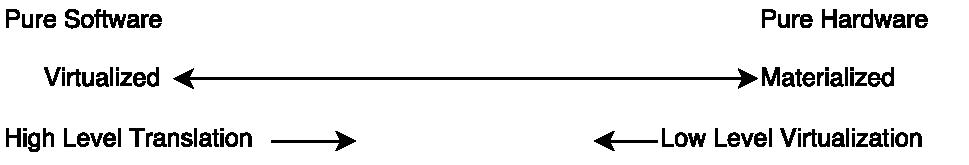
\includegraphics[scale=0.75]{spectrum_base}
\caption{Execution environments for SDN applications can utilize a high level
and low level implementation methods. The sweet spot lies somewhere between
the two.}
\label{overview}
\end{figure}

To translate high level code to a target device's native instruction set, more
work has to be done by the compiler to support both the language and the
device. Knowledge of the targets architecture, including specialized hardware
accelerators, must be well defined in order optimize execution. However this
approach is not always ideal, especially in the domain of SDN where network
switch architecture varies greatly between vendors in terms of capabilities
and features. This contributes to a lack of generalization in modern networking
where end-users are typically only able to specify configuration settings. In
order to bridge the gap, hardware components can be abstracted to provide
low level access to resources available in the system. A suitable execution
environment would lie somewhere between these two, taking advantage of powerful
compilers that can lower high level code while also leveraging low level
resource interfaces raised from the hardware.

\section{Background}
\label{intro:bg}
Networking architecture has become the focus of many facets in computing with
an increased reliance on network data. As more and more devices become
connected and users produce and consume data at an ever-increasing rate, the
way we accommodate these needs in networking infrastructure has prompted the
need for change. In order to service the needs of users, network engineers
require more functionality from their equipment than basic switching and
routing. Their networks need to be more intelligent, and allow for more
powerful user generated network applications. Unfortunately conventional
network switching devices are fairly static and rigid, and do not provide the
means to network engineers to create custom applications that suit their
particular needs. A network switch is composed of two high level components, a
control plane and a forwarding, or data, plane. The control plane manages the
configuration and state of the device, as well as compiled application
tenancy; whereas the data plane is responsible for executing forwarding
behavior over network traffic flows in the system. These components are
tightly coupled which hinders how a network application might be able to
abstract their functionality. At the upper level, control plane management is,
more or less, a fairly open entity. Users can configure their networks and
applications running on them within the confines of the interface exposed by
that particular switch vendor. To apply changes made in the control plane,
which may alter the configuration of the data plane, usually the device must
be rebooted. Most changes made to resources used by the data plane and
applications can only occur when the system is starting up. This has much to
do with the fact that the applications running on these devices are created by
the vendors themselves, who understand the underlying architecture in the
system and are able to push the application logic down into the hardware. The
result is high performance networking applications, that utilize hardware
accelerators and are tuned for that particular system. However this comes at a
great cost, flexibility. Network engineers are at the mercy of networking
device manufacturers when they want to mold their network to suit their needs.
The data plane in a network switch remains a black box, with features and
capabilities varying greatly between vendors. This lack of transparency makes
it difficult to model an abstract machine that can be targeted by networking
applications.

Research in the domain of SDN investigates the
decoupling of the two planes, giving users the ability to create networking
applications that can respond to changes in network traffic flows in real time.
The emphasis in this model is to allow a single control plane to manage
numerous data planes in one or many switches as a unified entity. Most of the
work in this field revolves primarily around virtual network switches,
building on concepts provided by the OpenFlow specification \cite{openflow}.
We chose to focus on the implementation of a single programmable network
device, where the control and data plane exist within the same system. This
allowed us to produce a specification for an abstract machine for networking
applications. The machine defines memory and object models, program execution
semantics, a set of required operations, access to guaranteed resources, and
the types of objects that it operates on and their behaviors. It must also be
able to support a variety of high level programming languages as well as
platforms and network processor architectures. Optimization support for
specialized instruction execution and offloading computation to hardware
accelerators and/or co-processors is also a key requirement to keep
performance on par. Languages are able to interact with the virtual machine
through an application binary interface (ABI), that defines symbols and rules
that dictate how they can utilize the runtime system. This approach has
produced an instance of an abstract machine that provides the necessary
resources and capabilities required to support network application execution.


\section{Goals}
\label{intro:goals}
It is clear that there is need for runtime support for compiled
networking applications. The virtual machine needed to provide functionality
for both parts of a network switch, the control and data planes, and allow
applications to have control and access to these resources at the user level.
In addition to servicing the needs of applications, the runtime needs to be
supported on a variety of architectures and utilize the materialized and
abstracted resources available. Freeflow aims to fill the gap between high level
network programming languages and low level switch architectures for the purpose
of SDN.

\section{Contributions}
\label{intro:contrib}
The contributions presented in this thesis come from numerous experiments with
low level networking hardware. These experiments helped characterize the
problem domain with respect to low level abstraction of network interfaces and
high level language translation to a native instruction set architecture
(ISA). The culmination of lessons learned are found in the Freeflow virtual machine (FFVM) implementation, the main focus in this work. The experiments evaluated include:

\begin{itemize}
  \item DPDK - Low level port abstractions
  \item Netmap - Low level port abstractions
  \item RISC-V - Native instruction execution
\end{itemize}

% \subsection{Virtual Machine}
% \label{intro:vm}
% FFVM is a process that provides the resources necessary for network
% applications to execute. These resources are:
%
% \begin{itemize}
% \item \emph{Ports} - The source of I/O for applications.
% \item \emph{Tables} - Matching data structures that define forwarding behavior.
% \item \emph{Packet Context} - Contextual information about a packet.
% \item \emph{Action Exection} - Native FFVM instructions to be executed by the
% runtime.
% \item \emph{Memory} - Packet Context buffers.
% \item \emph{Threading} - Infrastructure for modeling applications in various
% threading architectures.
% \end{itemize}
%
% \subsection{Runtime Support Library}
% \label{intro:rsl}
% Freeflow provides a runtime support library that Steve applications can
% leverage to execute as efficiently as possible. The library houses a collection
% of system calls, exposed as external C functions, to allow applications to call
% into the system during execution. These system calls allow the runtime to map
% the execution of certain instructions to the most appropriate computational
% device present and provide access to guaranteed resources.

\section{Organization}
\label{intro:map}
% Related works are contained in the Chapter \ref{related}, detailing some of the
% more mature research efforts in the domain of SDN, and other overlaping problem
% domains.
The thesis is organized as follows. In Chapters \ref{hardware} and \ref{insn}, the early investigations into
hardware abstraction and processing instructions are discussed,
respectively. This section journals the different approaches that were
considered in the design and implementation throughout this project, and
explains the benefits, deficits, and lessons learned from each approach.
Chapter \ref{ff} covers the design and implementation of the Freeflow system,
including application hosting, the virtual machine, the runtime support
library and the application binary interface exposed. This chapter discusses
the details of the contributions made towards this work at length.
Chapter \ref{expr} presents the experiments conducted as well as some initial
evaluation metrics collected. These demonstrate basic networking device
functionality for emulating Ethernet port end-points and cross-connects over
TCP sockets, and provide a baseline which can be used to further optimize the
system.
In the final chapter, Chapter \ref{concl}, the conclusions drawn from the
research conducted are discussed. Future work with respect to lessons learned
throughout the development of this project and integration with other SDN
programming languages and frameworks are also covered.

% Lastly, Appendix \ref{abi-listing} contains a listing of the ABI provided by
% the Freeflow virtual machine as a reference.

\chapter{RELATED WORK}
\label{related}
The related works section is comprised of the more current projects being
developed in this problem domain, SDN.

\section{Software Defined Networking}
\label{related:sdn}
SDN provides a networking device model where the control and data planes are
decoupled from one another, where a single control plane is responsible for
distributing application execution across a set of network switches viewed as
a unified data plane instance. Applications generally operate at the control
plane level and rely on distributed platforms, such as OpenVSwitch (OVS)
\ref{ovs}, to push the logic down to the hardware level. Generally a hypervisor
sits on top of each switch and helps orchestrate the entire system.


\section{Networking Applications}
\label{related:apps}
Not all networking applications operate in the same conceptual space, that is,
they generally act as a part of a larger system. Applications can operate on a
particular traffic flow, a node within a network, or across the entire network.
% Add more to this.

\section{OpenFlow}
\label{related:of}
% Add more to this.
The OpenFlow \cite{openflow} model defines a messaging layer that the control and, potentially
distributed, data plane(s) can communicate through. This is embodied in the
OpenFlow Protocol, which specifies a set of ``instructions'' that the control
and data planes must support.

\section{DPDK}
\label{related:dpdk}
Intel's Data Plane Development Kit (DPDK) \cite{dpdk} provides a framework that
allows programmers to create highly optimized data plane applications.

\section{Open Data Plane}
\label{related:odp}
Talk about this a little bit.

\section{Open Virtual Switch}
\label{related:ovs}
Open Virtual Switch (OVS)
\begin{figure}[h]
\centering
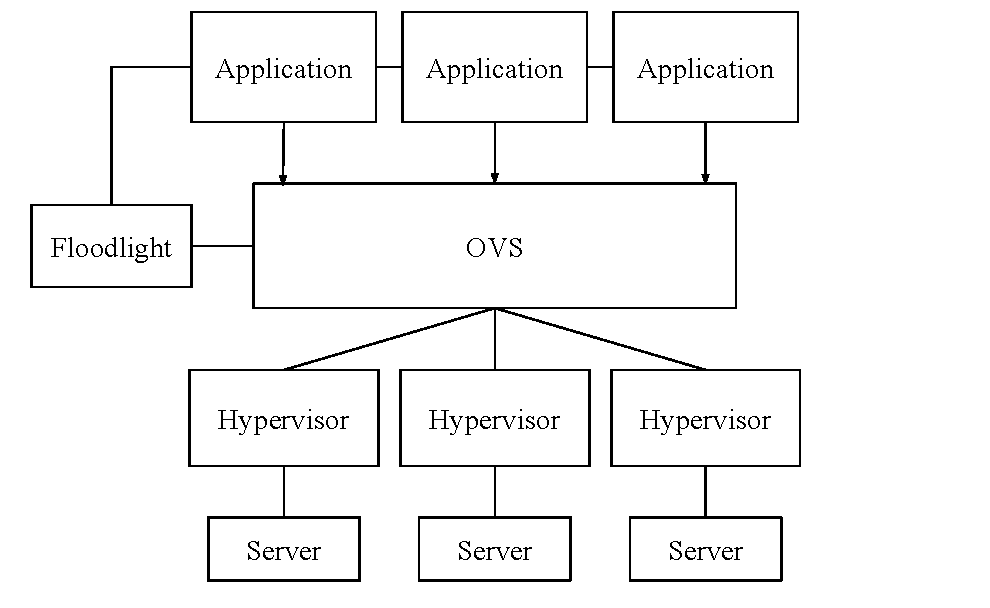
\includegraphics[scale=0.5]{ovs_arch}
\caption{The OpenVSwitch architecture.}
\label{related:ovs_arch}
\end{figure}

\section{NetASM}
\label{related:netasm}
Talk, at length, about netasm. Can bring up riscv here too.

\subsection{RISC V}
% Rewrite this.
Our next approach focused more on the interaction between the language and
runtime components of our system, with the hopes of being able to execute
the language in a native ISA. We came across an extensible ISA, RISC V, that
provided not only basic arithmetic, logical, and control flow instructions but
also left room for a number of custom instructions. This seemed like a great
way to incorporate specialized network programming instructions into a native
format. Unfortionately, this would also require that we interpret and implement
all of the supported instructions in the set in an virtual machine. As a result
the execution took a serious hit in terms of performance at the cost of this
flexibility. This project requires a fine balance of flexibility and
performance, and the deviation between these properties was too great.

\section{Heterogenous Compute Platforms}
\label{related:hcp}
Discuss the heterogenous compute models considered.

\subsection{Heterogenous System Architecture}
\label{related:hcp:hsa}
Or HSAIL \cite{hsail} provides a specification for creating a heterogeneous
system architecture that

\subsection{Open Compute Language}
\label{related:hcp:ocl}
Open Compute Language.

\subsection{CUDA}
\label{related:hcp:cuda}
Compute Unified Device Architecture.

\section{Frameworks}
\label{related:frameworks}
Discuss the frameworks considered.

\subsection{Seastar}
\label{related:frameworks:seastar}
Bad ass, if you've got the HW to support it.

\subsection{Libevent}
\label{related:frameworks:libevent}
Very complicated, not easy to target custom backends (dpdk).

\chapter{ARCHITECTURE}
\label{arch}

\section{Port}
\label{arch:port}

\section{Processor}
\label{arch:proc}

\subsection{Accelerator}
\label{arch:proc-accel}

\section{Controller}
\label{arch:controller}

\section{Data Plane}
\label{arch:dataplane}

\section{Application}
\label{arch:app}

\chapter{FREEFLOW}
\label{ff}
In this chapter we discuss the Freeflow programmable virtual switch
implementation details. The first few sections describe the higher level 
components in this architecture, the control and data planes, applications, as 
well as the virtual machine. Then we dive into the details of the object 
models (e.g. ports, tables, and the packet context), native instruction 
execution semantics, as well as the memory and threading models currently 
supported.

\begin{figure}[h]
\centering
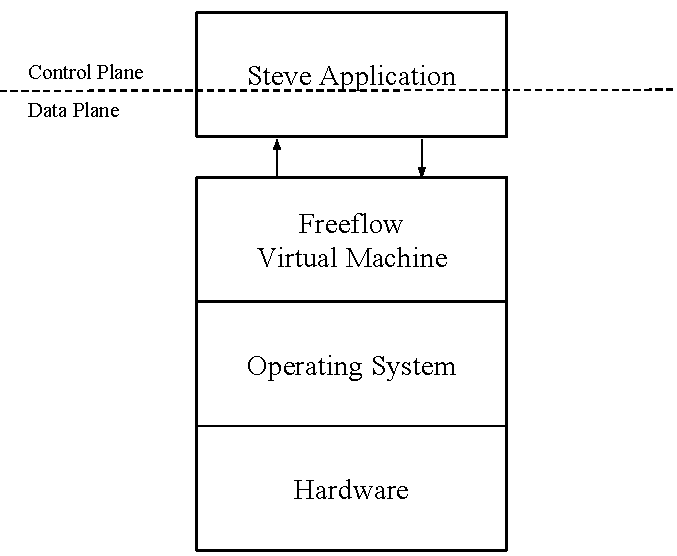
\includegraphics[scale=0.5]{ff_arch}
\caption{The Freeflow System Architecture.}
\label{ff_arch}
\end{figure}

\section{Control Plane}
\label{ff:cp}
The control plane acts as the brain in a network switch, and is responsible for
the hosting of applications as well as the management of the underlying data
plane. In the control plane, the system configuration establishes the resources
that must be provided to support application execution. During execution, 
events raised from the data plane are caught and processed by application 
defined event handlers.

\section{Data Plane}
\label{ff:dp}
A data plane executes the forwarding behavior for traffic flows using a variety
of hardware, and sometimes software, constructs available in a given system.

\section{Applications}
\label{ff:app}
Freeflow applications provide the logic for the control and data planes in the
switch. This is a departure from common SDN paradigms, where the two planes are
treated as seperate entities and communicate over a secure channel. The reason
for blurring the line between the two parts is to reduce the overhead penalty
that is incurred in the former model. By allowing the application to straddle
the line between the control and data planes, the logic it provides is able
to be pushed into hardware and executed in a native fashion.

Networking applications operate on packets, utilizing information found inside of nested protocol headers to determine the appropriate action to take. 

\section{Packet Context}
\label{vm:packet-context}
Network packets are arranged as nested protocol headers, which contain fields that describe the structure and contents of a particular layer. Since the Freeflow data plane has no knowledge of any protocol structures (i.e. it is protocol independent), it operates on contextual information extracted by applications and stored in a \emph{context} object. The metadata contained in a context allows the data plane to provide robust network functionality and execute a variety of network applications.

\subsection{Packets}
In networking, packets represent raw data that has been transmitted over some media with protocol headers for each layer contained in the packet. Each layer gives information about the current


\begin{figure}[h]
\centering
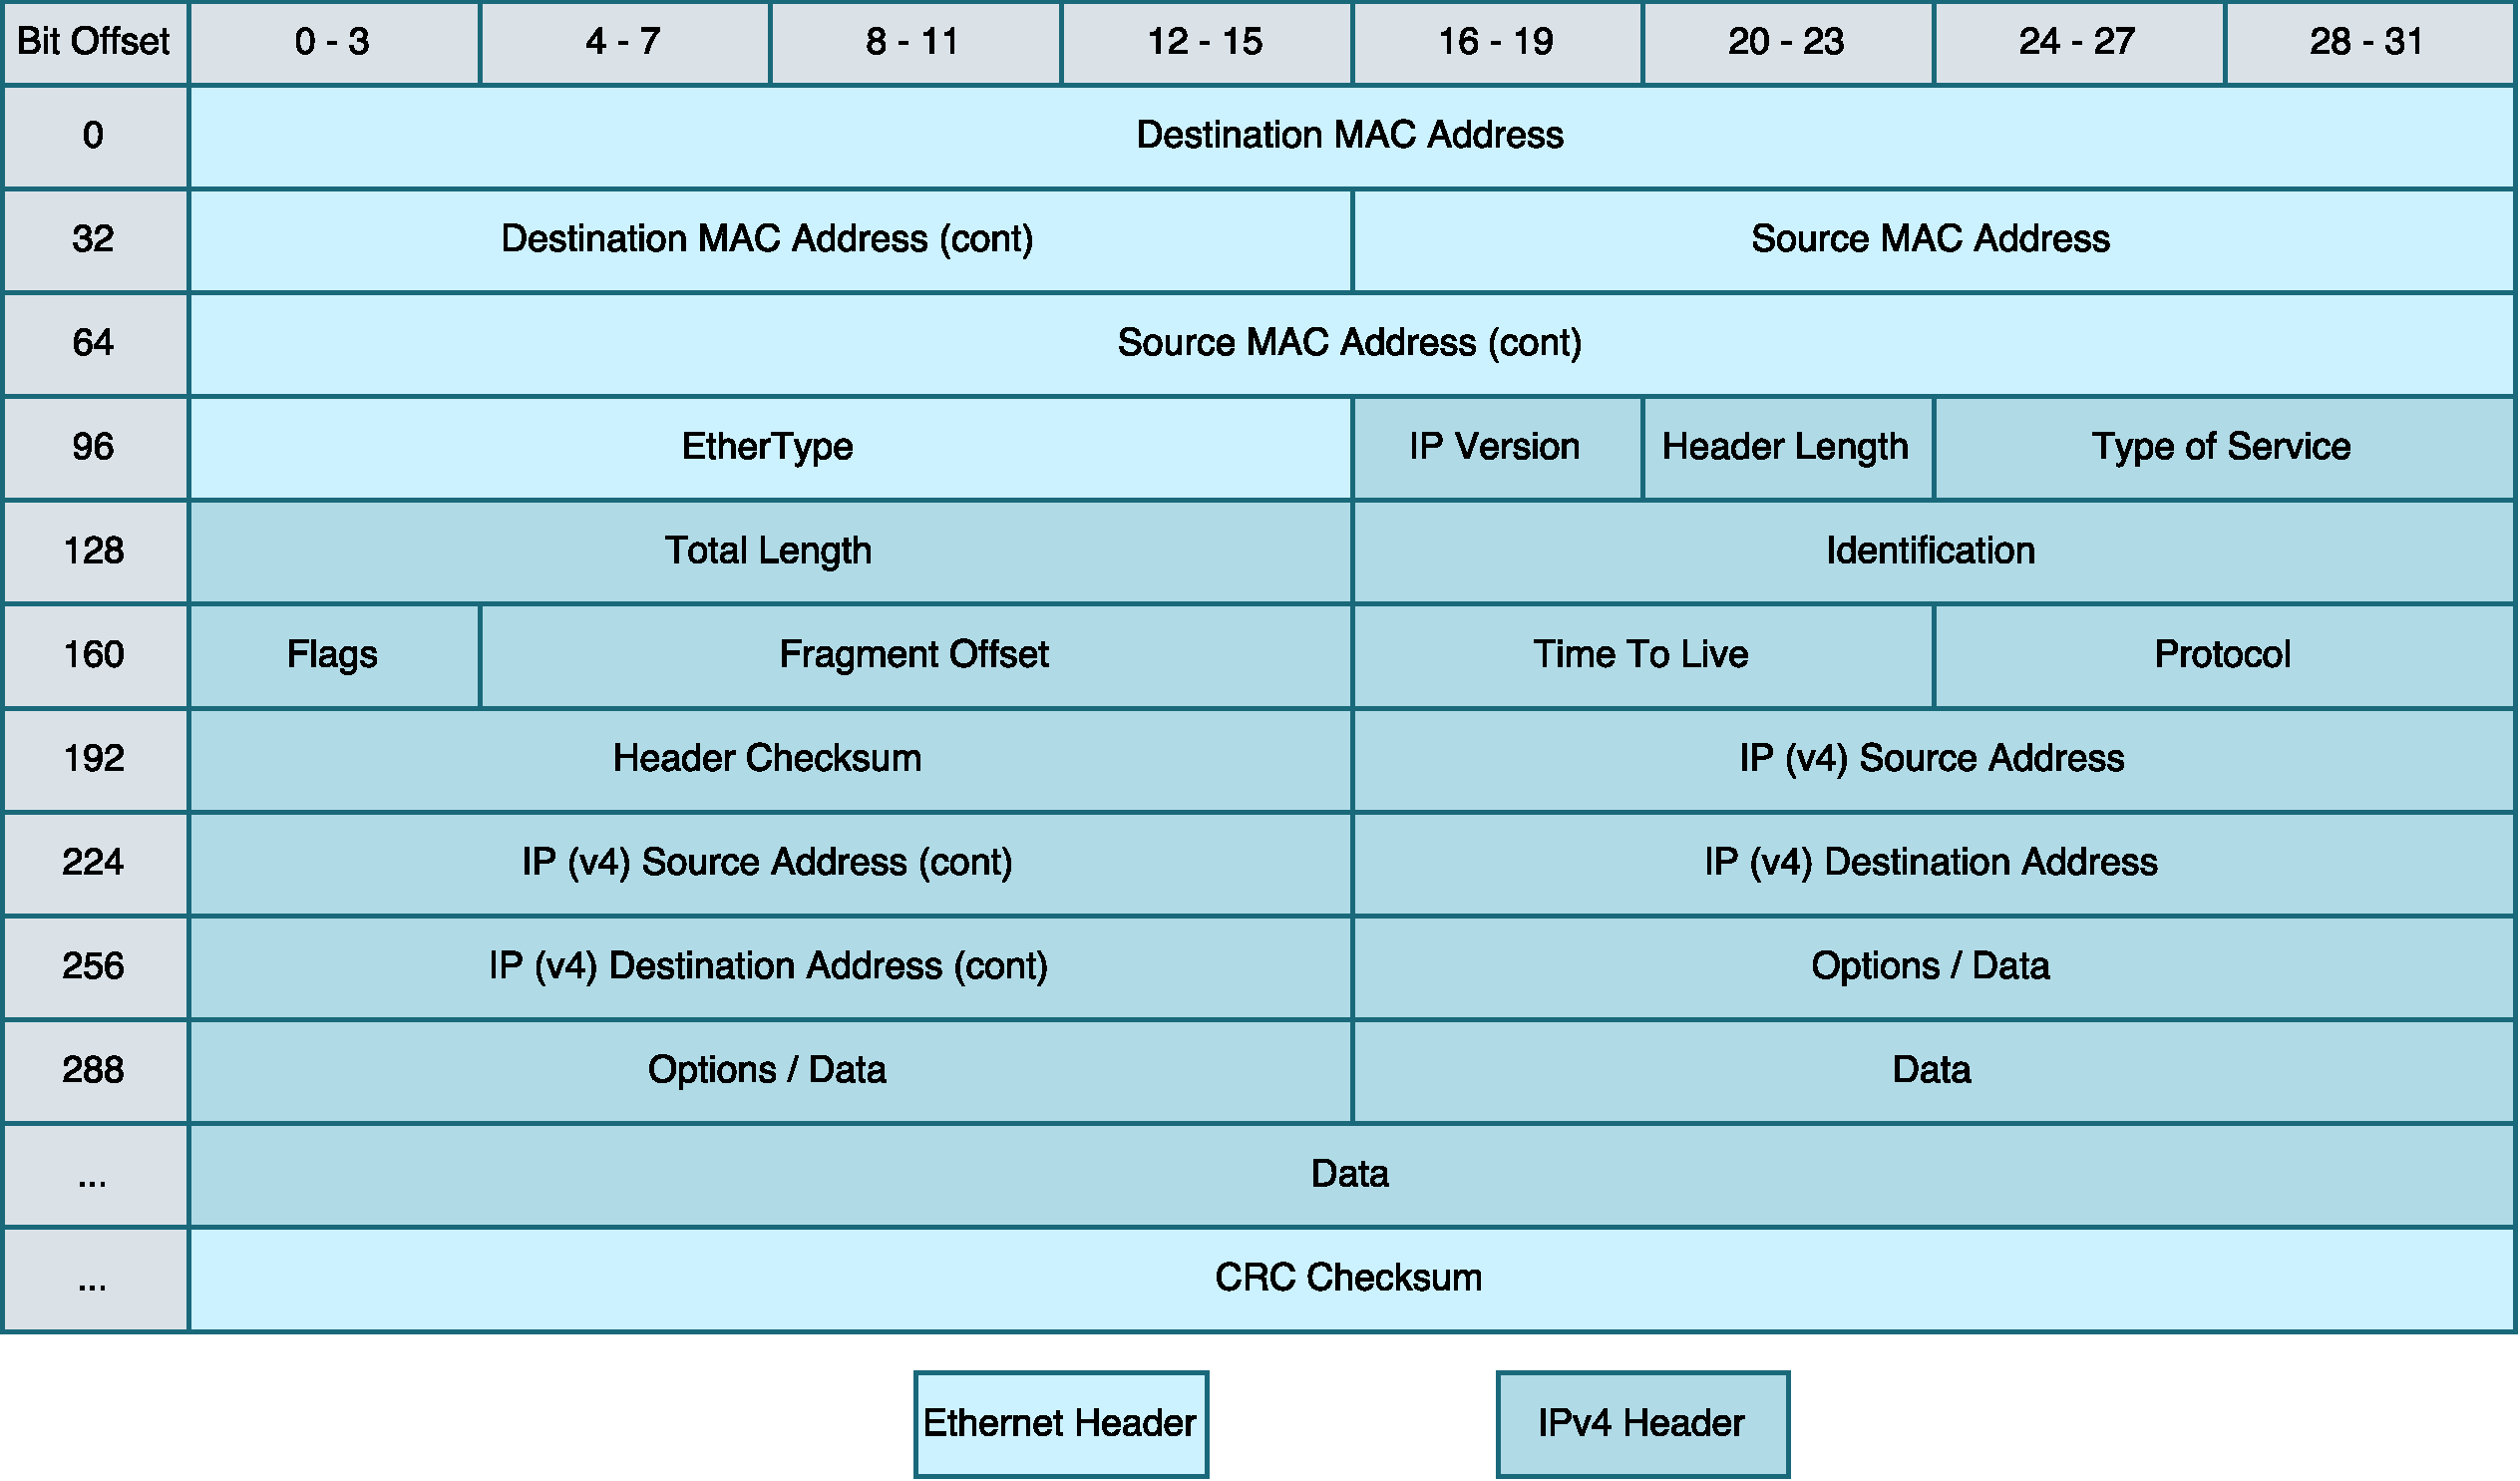
\includegraphics[scale=0.33]{ipv4_eth_frame}
\caption{An IPv4 Ethernet frame.}
\label{fig:ipv4_eth_frame}
\end{figure}

\subsection{Context}
Stuff about context structure, etc.

\begin{lstlisting}[language=c++]
struct Decode_info {
	uint16_t 		pos;	   // Packet decoding offset
	Environment headers; // Saved packet header locations
	Environment fields;	 // Saved packet fields locations
};

struct Context {
	Ingress_info input;
	Control_info ctrl;
	Decode_info	 decode;
	Packet 			 packet;   // A handle to packet memory
	Metadata 		 metadata; // Application-defined metadata
	Action_list	 actions;  // A sequence of instructions
};
\end{lstlisting}

\begin{figure}[h]
\centering
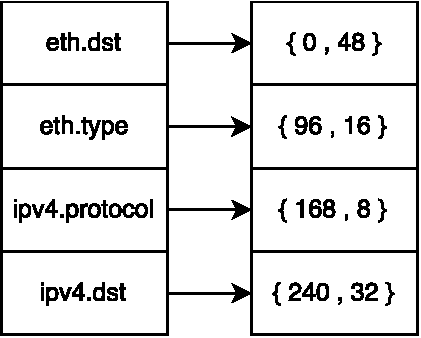
\includegraphics[scale=0.5]{context_concrete}
\caption{An example binding environment for an IPv4 Ethernet frame.}
\label{fig:context_binding}
\end{figure}

\section{Virtual Machine}
\label{vm}
The Freeflow Virtual Machine is composed of modular parts that a programmer can
assemble into a virtual switch.

\begin{figure}[h]
\centering
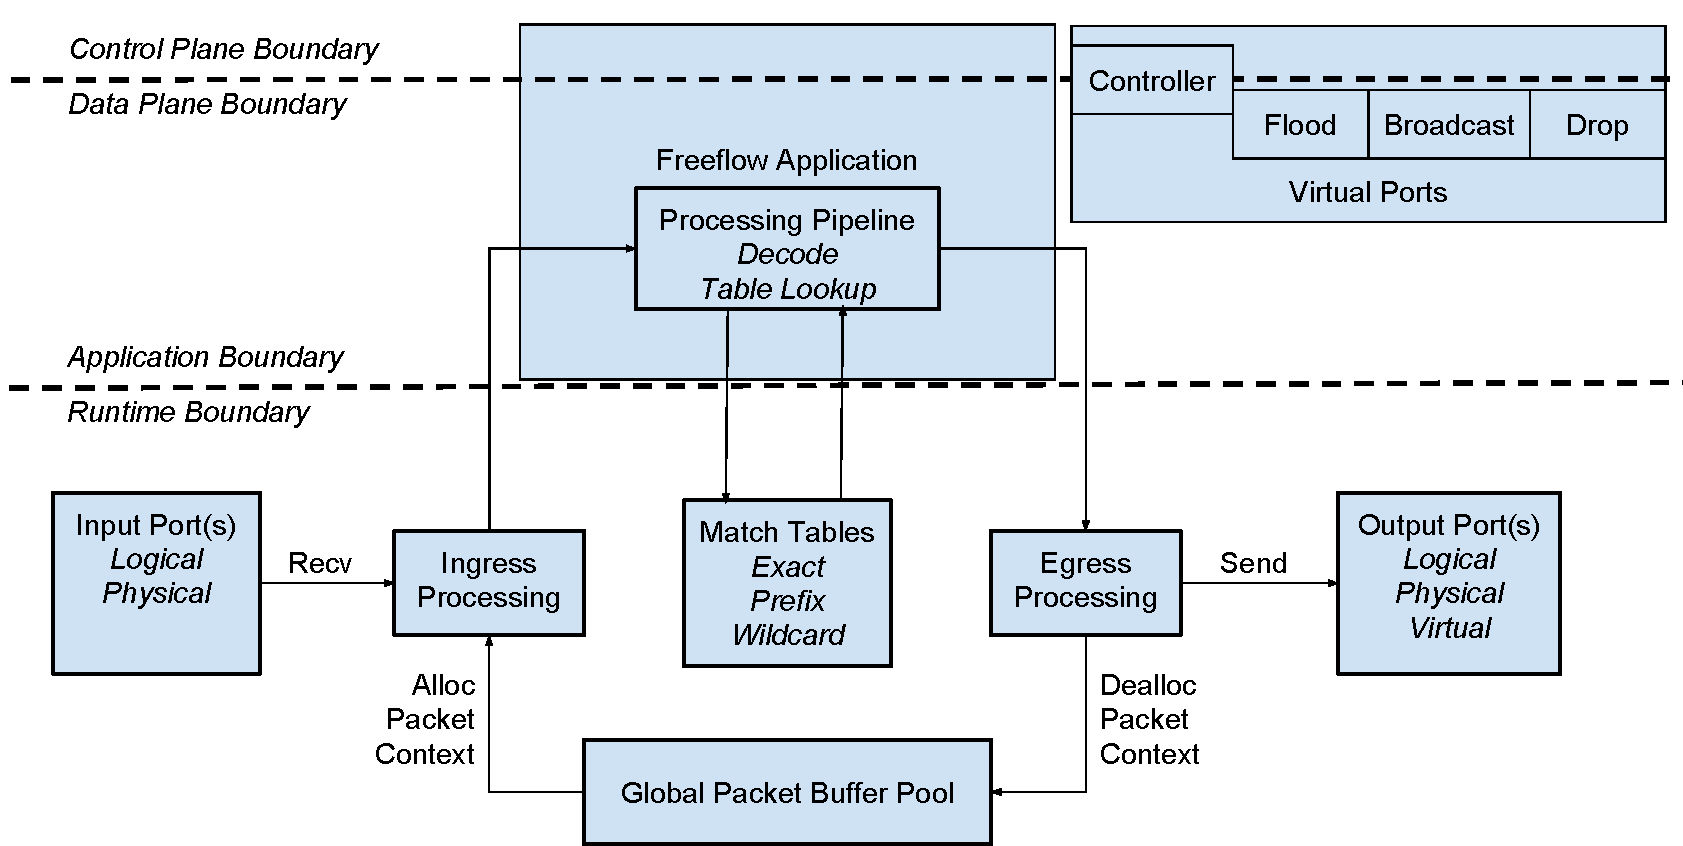
\includegraphics[scale=0.5]{ff_system}
\caption{The Virtual Machine System Architecture}
\label{fig:ff_system}
\end{figure}

\section{Ports}
\label{vm:port}
Ports act as the main source of I/O for network applications. The provide the
means to receive and send packets that are entering and leaving the system. As
an abstract type, the port interface is fairly simple. Any derived port object
needs to implement the following four functions:

\begin{itemize}
\item Send - Transmit packet data.
\item Receive - Retrieve packet data.
\item Up - Puts the port into a usable state, data can be sent and received.
\item Down - Disables port functionality.
\end{itemize}

Port objects can be classified as being either physical, logical, or virtual. A
physical port represents a hardware networking interface, e.g. ethernet cards.
Logical ports represent software networking constructs that utilize file
descriptors to act as a endpoint for communication. An illustration of the port
object UML can be found in figure \ref{port_uml}. Virtual ports are derived
from logical ports, and provide specialized functionality for the system. To
further classify the port type, they can be either seen as an \emph{input} 
port, where data from an external source can be injected into the system, or an
\emph{output} port, which sends data to other external or internal devices.

\begin{figure}[h]
\centering
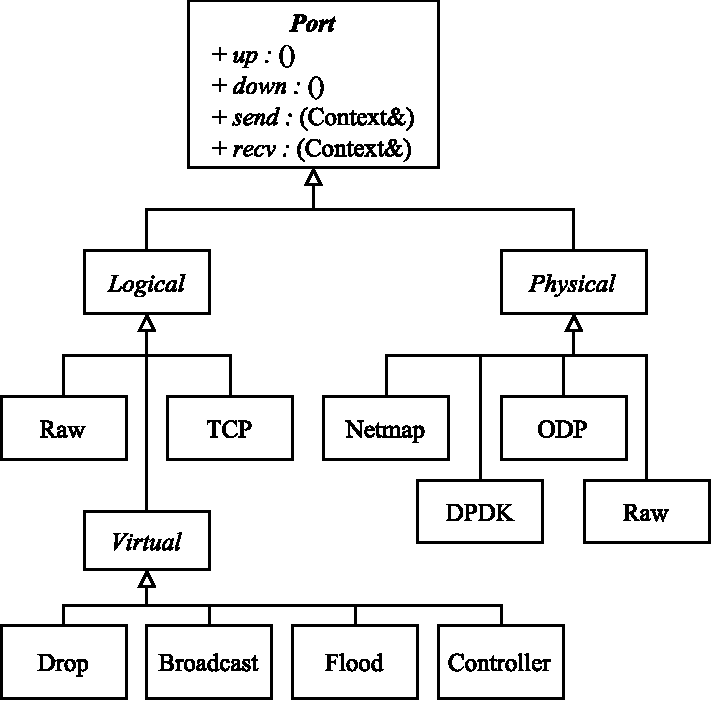
\includegraphics[scale=0.65]{ff_port_uml}
\caption{Freeflow port uml diagaram.}
\label{port_uml}
\end{figure}

\section{Tables}
\label{vm:tables}
In network switches, tables are used to match properties from network flows 
with user-defined forwarding behaviors. They can be defined using a variety of
data structures and algorithms to implement them, but generally are categorized
as \emph{exact}, \emph{prefix}, or \emph{wildcard}. Each entry in a flow table
contains a \emph{key}, that is compared to a certain field within packet

Entries in a table contain a \emph{key}, which is used to aggregate traffic 
containing similar characteristics into flows.


\section{Instructions}
\label{vm:insn}
Native insn execution. Offloading, optimizations.

\section{Memory}
\label{vm:memory}
Memory model.

\section{Threading}
\label{vm:threading}
Threading models.

\chapter{FREEFLOW}
\label{ff}
The Freeflow project aims to bridge the gap between high level network
programming languages and low level networking hardware by defining an ideal
execution environment for network applications. Evaluating the benefits and
deficits with respect to flexibility and performance provides a more accurate
level of translation or abstraction to use. In Figure \ref{ff_arch}
the Freeflow system architecture is illustrated.

\begin{figure}[h]
\centering
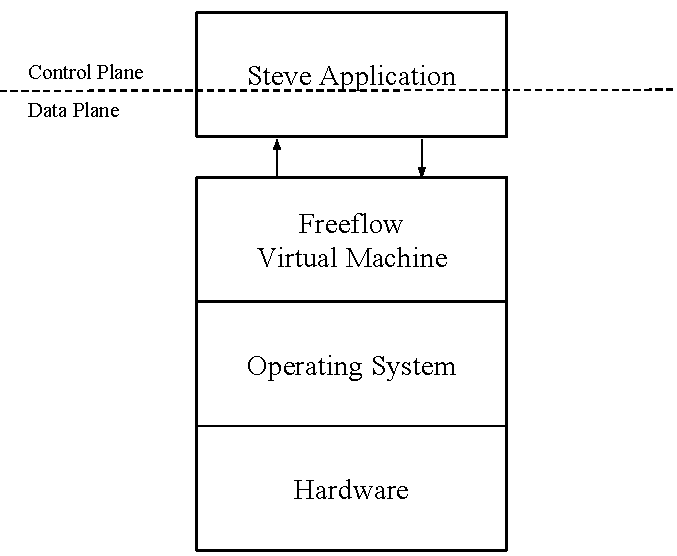
\includegraphics[scale=0.5]{ff_arch}
\caption{FFVM provides computational and memory resources to applications.}
\label{ff_arch}
\end{figure}

This chapter elaborates on the Freeflow programmable virtual switch
implementation details. The first few sections describe how applications are
hosted and how packet data is represented and manipulated. In the remainder of
the chapter, the virtual machine and its components are discussed. These include
object models for ports and tables, dynamic instruction execution, as well as
the memory and threading models supported.

% \section{Control Plane}
% \label{ff:cp}
% The control plane acts as the brain in a network switch, and is responsible for
% the configuration and management of the underlying data plane. In an FFVM
% virtual switch, control logic is provided by a hosted network application that
% is dynamically loaded. The application
%
% In the control plane, the system configuration establishes the resources
% that must be provided to support application execution. During execution,
% events raised from the data plane are caught and processed by application
% defined event handlers in the controller.
%
% \section{Data Plane}
% \label{ff:dp}
% A data plane executes the forwarding behavior for traffic flows using a variety
% of hardware, and sometimes software, constructs available in a given system. The
% FFVM data plane provides the necessary resources to host compiled network
% applications.

\section{Application Hosting}
\label{ff:app}
Freeflow applications provide the logic for the control and data planes in the
switch. This is a departure from common SDN solutions, where the two planes are
treated as separate entities and typically distributed across many devices.
The reason for blurring the line between the two parts is to reduce the overhead
penalty that is incurred in the former model. By allowing the application to
straddle the line between the control and data planes, the logic it provides is
able to be pushed into the appropriate hardware and executed efficiently.

\begin{figure}[h]
\centering
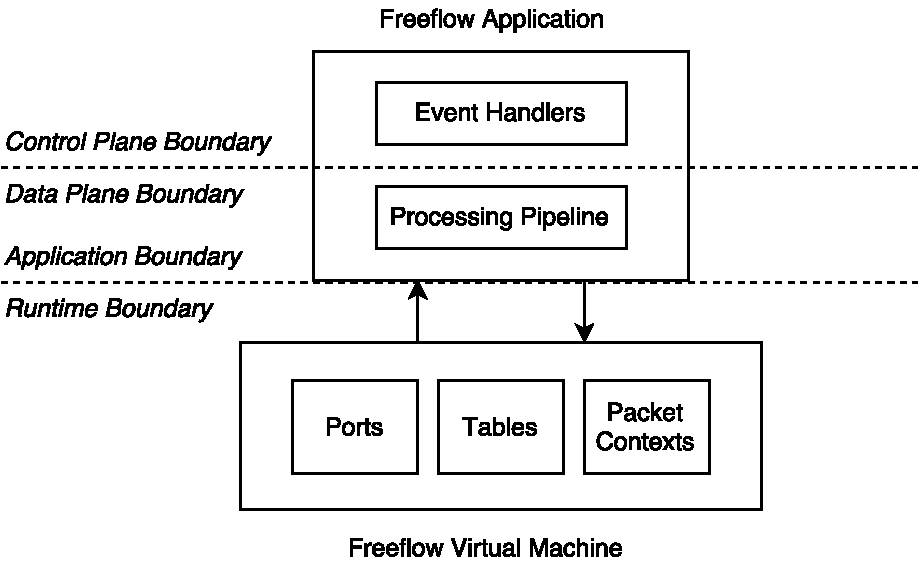
\includegraphics[scale=0.5]{application}
\caption{Freeflow application logic spans across the control and data plane
boundary.}
\label{app}
\end{figure}

Networking applications operate on packets, utilizing information found inside
of nested protocol headers to determine the appropriate action to take. In
Freeflow, applications and the virtual machine operate on packet contexts
that store contextual information about a packet in the system. Applications
use these contexts to process packets in a series of stages that extract
protocol information and apply rule matching logic to them. A typical
application pipeline is illustrated in Figure \ref{app_pipeline}.

\begin{figure}[h]
\centering
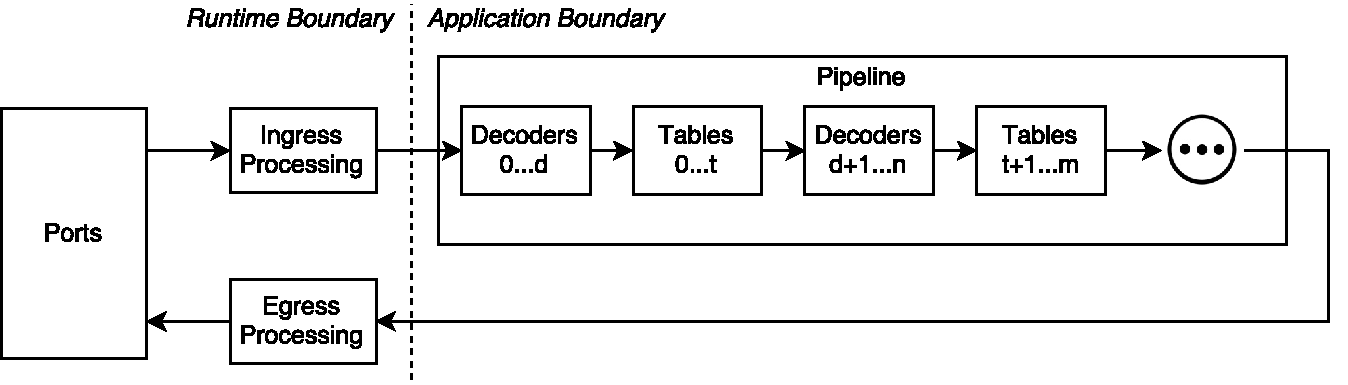
\includegraphics[scale=0.5]{app_pipeline}
\caption{A Freeflow application defines a list of decoders and tables.
Each decoder extracts values from a packet which are used in table lookups.}
\label{app_pipeline}
\end{figure}

Freeflow applications are loaded dynamically through application binary
files, compiled to native shared object libraries. Currently only one instance
of an application binary can be loaded into a FFVM process space. The FFVM
calls functions, exported as symbols from the binary, to manipulate the state
of the application. Freeflow application state is defined as:

\begin{itemize}
  \item \texttt{init} - All exported symbol handles have been resolved.
  \item \texttt{ready} - The application is loaded and able to start.
  \item \texttt{running} - The application is being executed.
  \item \texttt{stopped} - The application is halted.
\end{itemize}

The functions that control the application life cycle all require a handle
to the host data plane in order to provide dynamic allocation of resources.
These functions are:

\begin{lstlisting}
    ff_load(dp);
    ff_unload(dp);
\end{lstlisting}

The \texttt{ff\_load} function initializes global data plane resources required
by the application, such as tables. When successful the application state is
set to ``ready'', or is left in an ``init'' state when errors occur. During
FFVM tear down, a call to \texttt{ff\_unload} will release the allocated
resources if the application is not in a ``running'' state.

\begin{lstlisting}
    ff_start(dp);
    ff_stop(dp);
\end{lstlisting}

Applications ``learn'' about state and configuration changes to the data plane
they are hosted in through events. The \texttt{ff\_start} function sets the
application state to ``running'', starting packet processing and allowing events
to be handled. A call to start is only valid when the state of the application
is ``ready'' or ``stopped''. The \texttt{ff\_stop} function halts packet
processing, disables event handlers, and sets the state to ``stopped''.

\begin{lstlisting}
    ff_process(cxt);
\end{lstlisting}

The application defines the forwarding behavior for a data plane by providing
a packet processing pipeline. After a packet is received and exits ingress
processing, the FFVM calls the process function on a packet context. In order
to forward packets, the application must provide the definition of a packet
processing pipeline for the FFVM to execute.

\section{Packet Context}
\label{vm:packet-context}
Network packets are arranged as nested protocol headers, which contain fields
that describe the structure and contents of a particular layer. Since the
Freeflow data plane has no knowledge of any protocol structures (i.e. it is
protocol independent), it operates on contextual information extracted by
applications and stored in a \emph{context} object. The meta data contained
in a context allows the data plane to provide robust network functionality
and execute a variety of network applications.

\subsection{Packets}
In networking, packets represent raw data that have been transmitted over some
media with protocol headers for each layer contained in the packet. Each header
gives information about the structure and state of the current protocol being
processed. Figure \ref{ipv4_eth_frame} shows an example Ethernet frame
(packet) containing an IP (v4) header.

\begin{figure}[h]
\centering
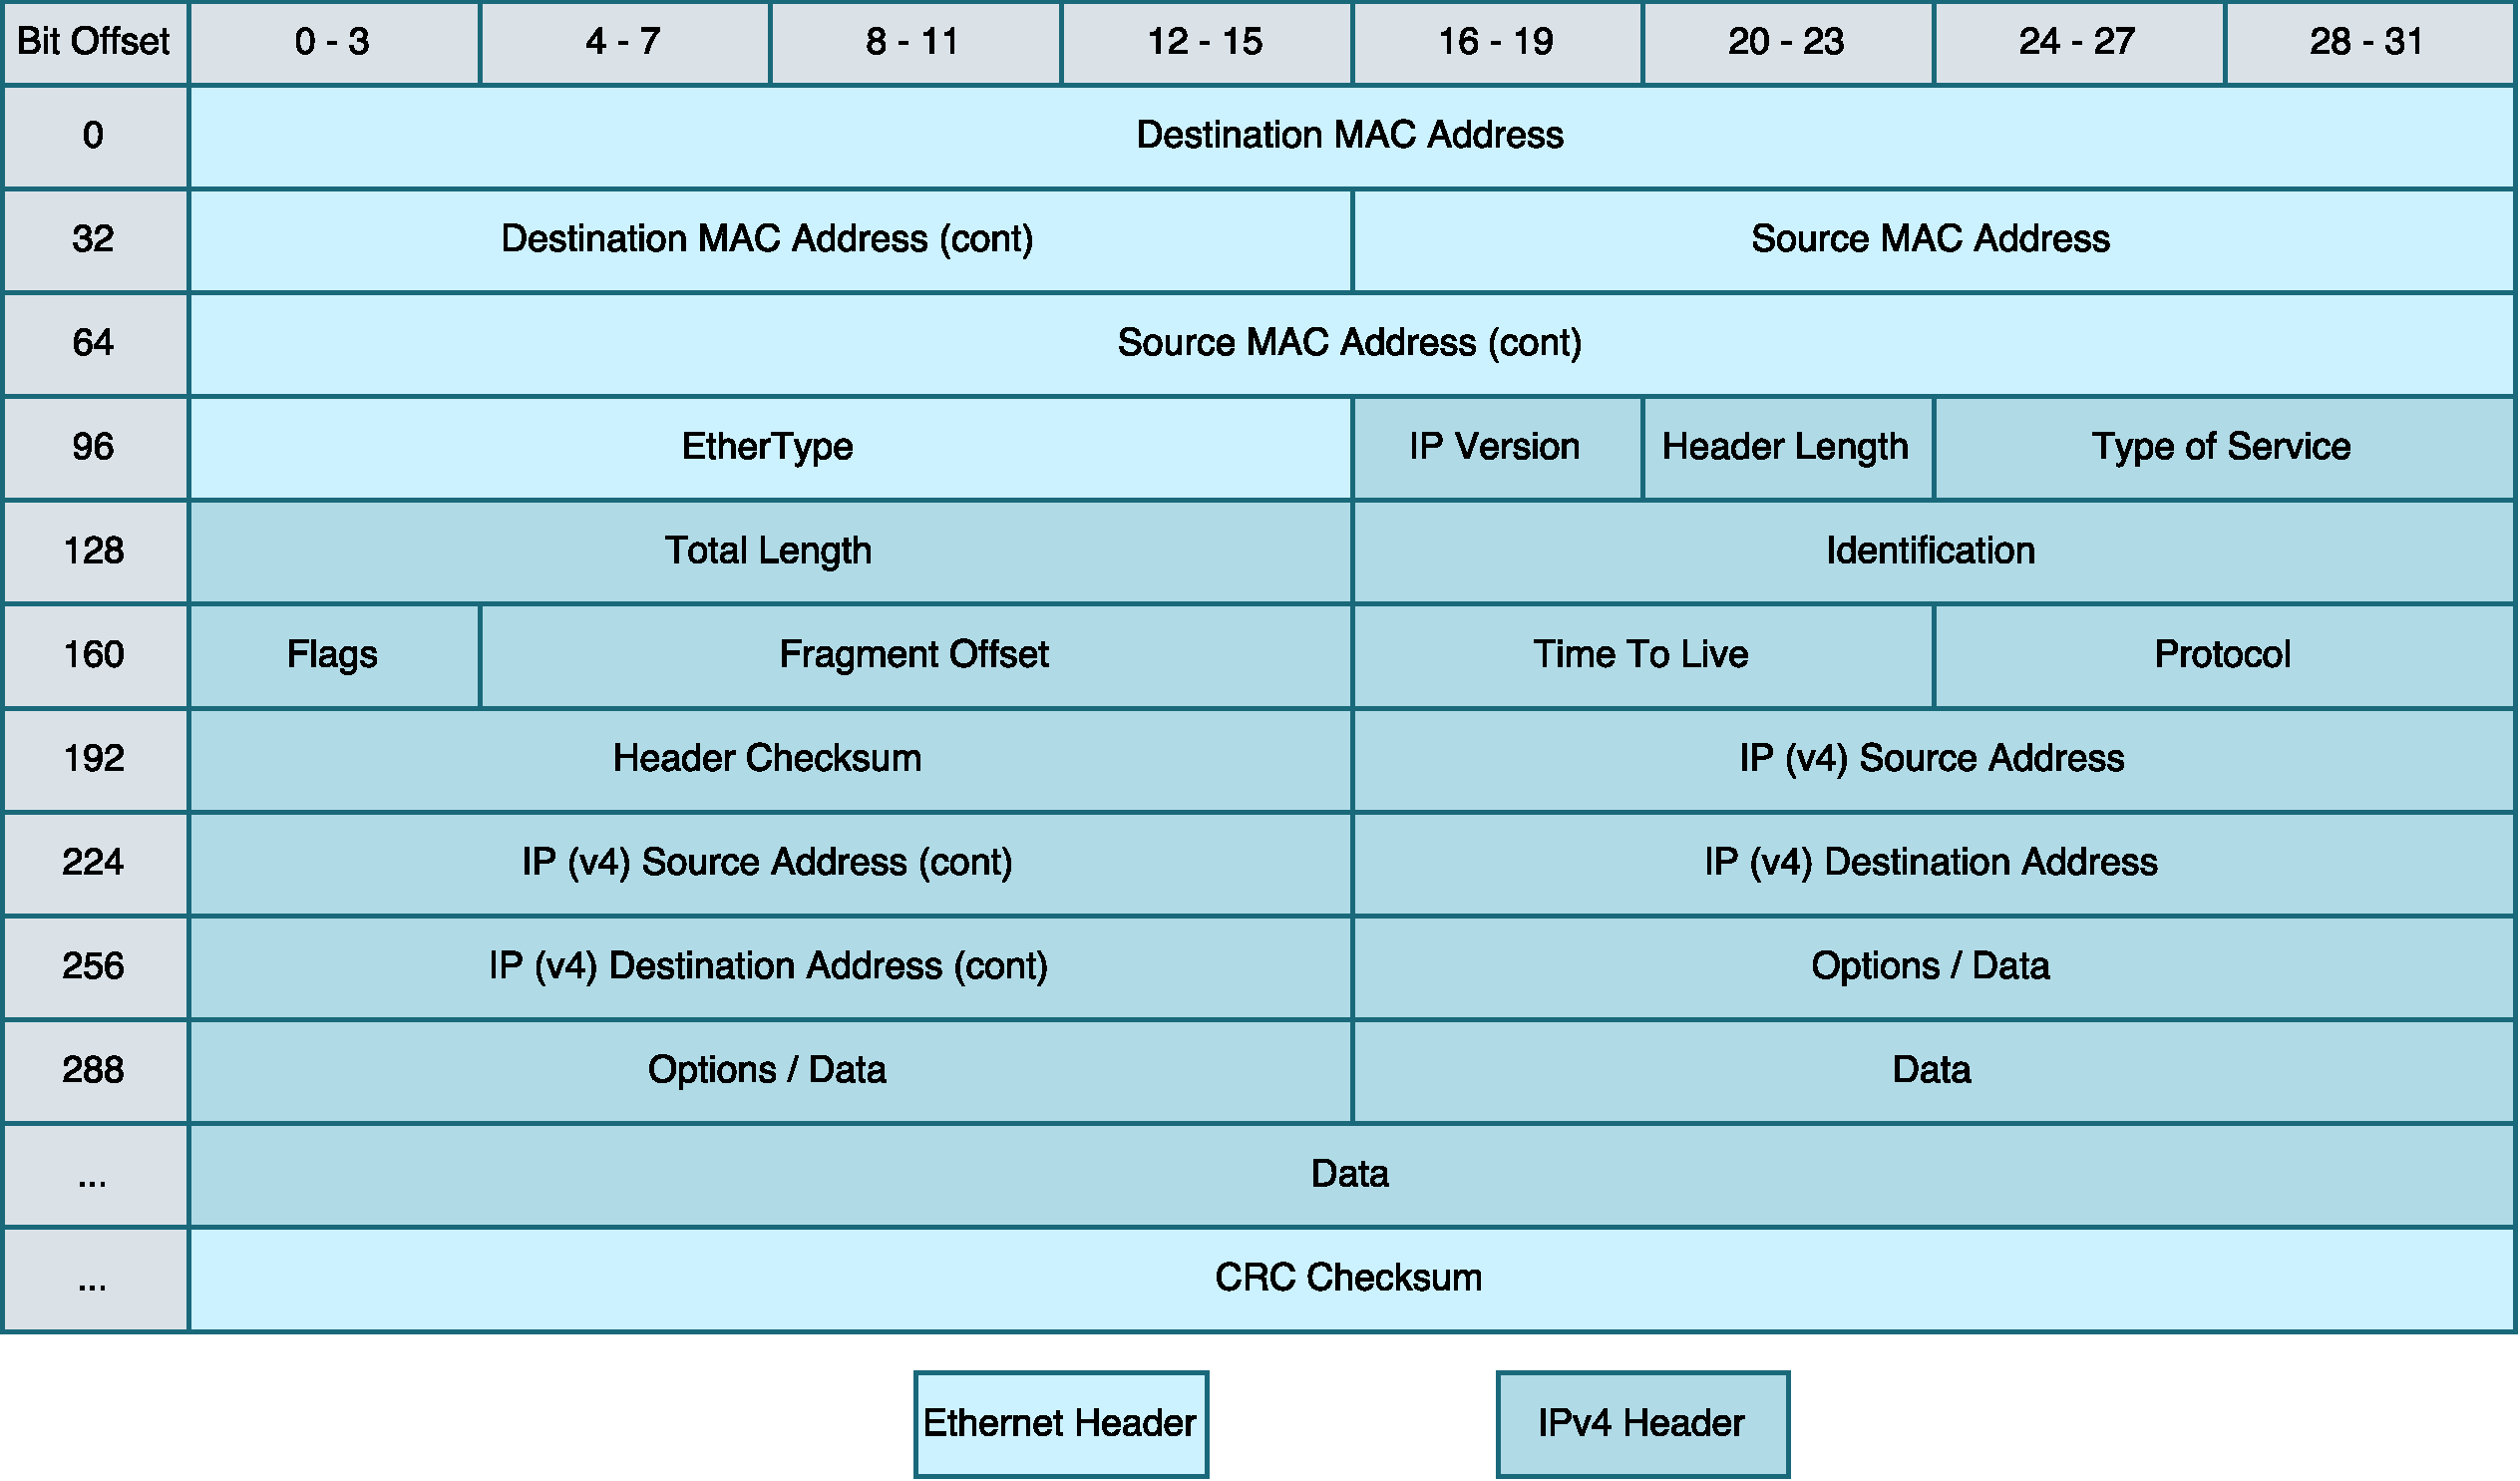
\includegraphics[scale=0.33]{ipv4_eth_frame}
\caption{An IPv4 Ethernet frame.}
\label{ipv4_eth_frame}
\end{figure}

The layout for each protocol is far from uniform, and fields within headers do
not always align to the traditional byte-aligned boundaries (e.g. Ethernet
MAC addresses which have a width of 48 bits). Storing these values in memory
results in wasted space, as larger data structures would need to be utilized.
Structure packing pragmas and bit width specifiers can be used to overlap
memory regions when the desired bit width is less than the standard width for
that type (e.g. \texttt{std::int\_64:48;}). However storing a copy of the
packet data would result in coherency issues, negatively impacting
performance. Instead the fields within headers are stored in a \emph{binding
environment}, discussed in the following section.

\subsection{Context}
The packet \emph{context} provides contextual information about an associated
packet in the system. A context is where applications store input, control, and
decoder information, as well as application meta data. This is also where they
build action lists.
Input information consists of data about the packets arrival into the system,
such as the input logical and physical ports. The control information maintains
the control flow of a context as it traverses processing pipelines.

\begin{lstlisting}
struct Decode_info {
  uint16_t    pos;     // Packet decoding offset
  Environment headers; // Saved packet header locations
  Environment fields;  // Saved packet fields locations
};

struct Context {
  Ingress_info input;
  Control_info ctrl;
  Decode_info  decode;
  Packet       packet;   // A handle to packet memory
  Metadata     metadata; // Application-defined metadata
  Action_list  actions;  // A sequence of instructions
};
\end{lstlisting}

As application packet decoders execute, they store the position, or offset, and
length of the desired fields as pairs in a binding environment, referred to as
the decode information. This environment notes the offset of a field within the
current protocol header, as well as the offset for each protocol header within
the packet buffer. Utilizing this heavy weight approach to referencing protocol
field information enforces a more precise data extraction plan and eliminates
coherency issues. Figure \ref{context_binding} shows the resulting binding
environment created after decoding the Ethernet source and destination fields,
as well as the IPv4 protocol and destination fields.

\begin{figure}[h!]
\centering
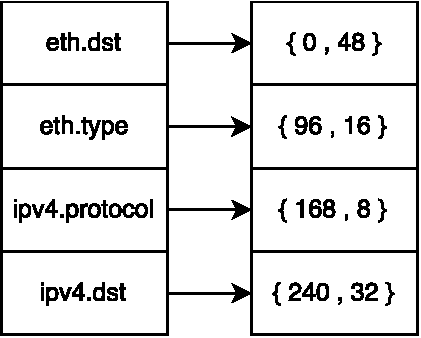
\includegraphics[scale=0.9]{context_concrete}
\caption{An example binding environment for an IPv4 Ethernet frame.}
\label{context_binding}
\end{figure}

The raw packet data is accessed through a handle held by the context. Depending
on the capabilities of the port that received the packet, this handle may point
to a Freeflow packet buffer or dedicated port memory. Meta data provides
``scratch'' space for applications to store additional information during
pipeline processing. The action list is composed of instructions that are to
be applied to a packet after exiting an application pipeline but before egress
processing. These instructions are used to modify fields within a packet, and
are explained further in Section \ref{vm:insn}.

\section{Virtual Machine}
\label{vm}
The Freeflow Virtual Machine is composed of modular parts that a programmer can
assemble into a virtual switch. This flexibility allows for the instantiation
of numerous switches with varying features and capabilities. In general,
switches require control and data planes as well as compiled network
applications to drive each component. A FFVM virtual switch can be assembled
by creating a data plane instance, in which port resources are added and an
application is loaded. User space drivers provision the machine with these
components and execute compiled applications. An example driver is shown in the
following listing.

\begin{lstlisting}
// Create a data plane instance named `dp1'.
ff::dataplane dp = ``dp1";

// Add virtual (internal) ports and two TCP sockets.
dp.add_virtual_ports();
ff::Port* port1 = new ff::Port_tcp(1);
ff::Port* port2 = new ff::Port_tcp(2);
dp.add_port(port1);
dp.add_port(port2);

// Load a sample application named `sample.app'.
dp.load_application(``sample.app");

// Set data plane configuration to `up',
// starting execution.
dp.up();
\end{lstlisting}

The driver makes a virtual switch with a single data plane, named ``dp1'', that
contains the predefined virtual ports and two TCP ports, with i.d.s 1 and 2
respectively. After allocating port resources, an application named
``sample.app'' is loaded, allowing the system to perform table configuration
and import the pipeline processing symbols. Figure \ref{ff_system} illustrates
the orchestration of the components utilized in the example driver listing.

\begin{figure}[h]
\centering
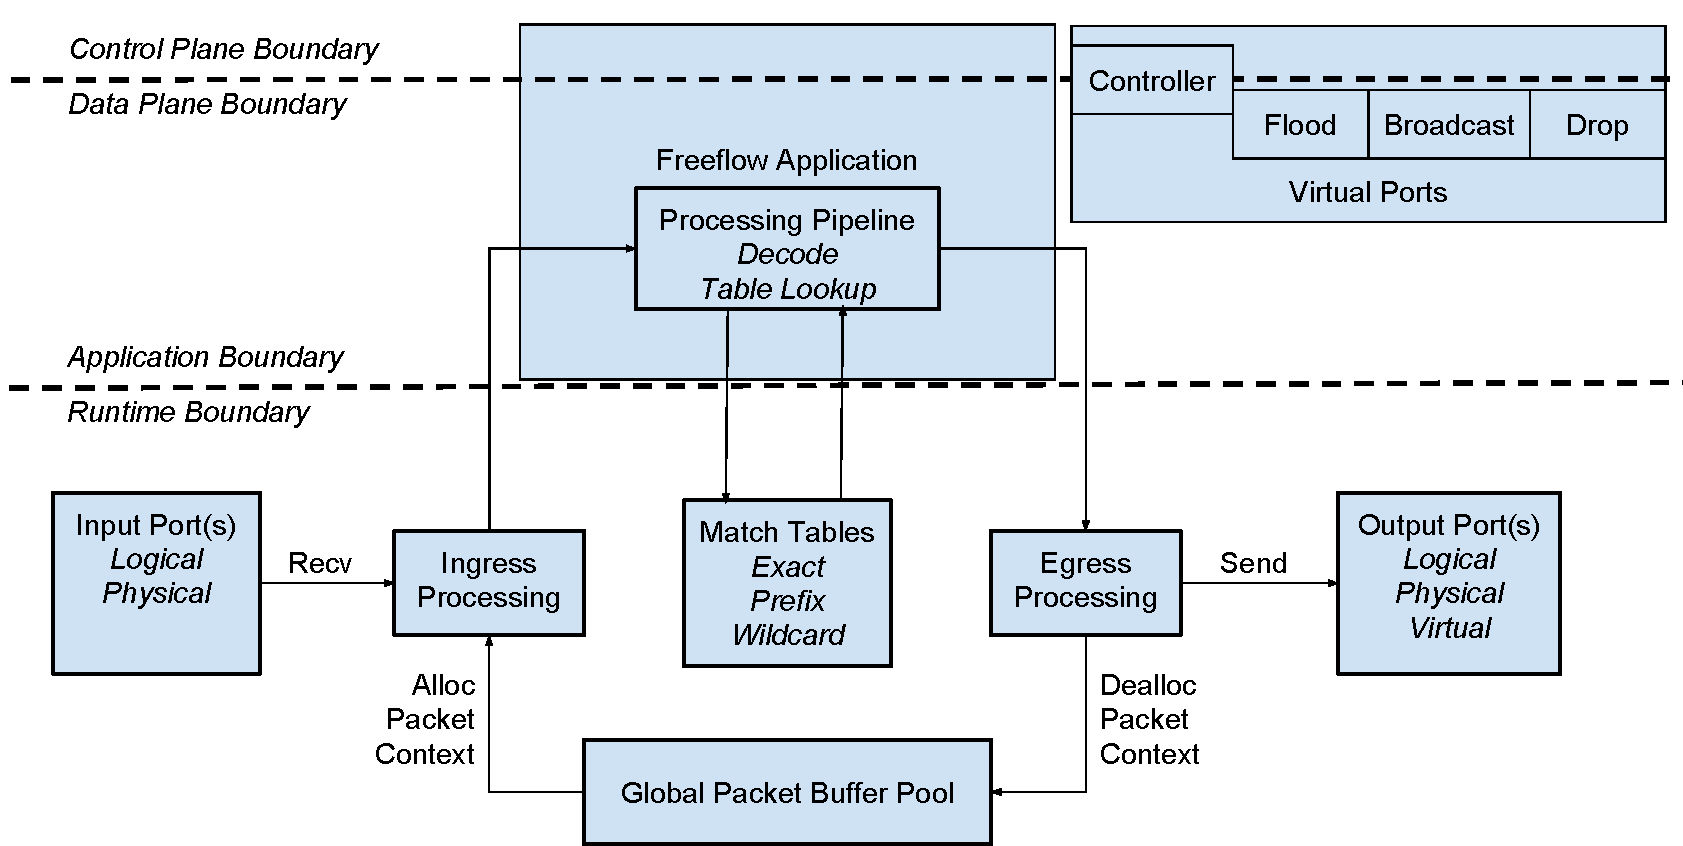
\includegraphics[scale=0.53]{ff_system}
\caption{The Freeflow virtual switch architecture.}
\label{ff_system}
\end{figure}

\section{Ports}
\label{vm:port}
Ports act as the main source of I/O for network applications. They provide the
means to receive and send packets that are entering and leaving the system. As
an abstract type, the port interface is fairly simple. Any derived port object
needs only implement the following four functions:

\begin{itemize}
\item Send - Transmit packet data.
\item Receive - Retrieve packet data.
\item Up - Puts the port into a usable state, data can be sent and received.
\item Down - Disables port functionality.
\end{itemize}

Port objects can be classified as being physical, logical, or virtual. A
physical port represents a hardware networking interface, e.g. Ethernet cards.
Logical ports represent software networking constructs that utilize file
descriptors to act as an endpoint for communication. An illustration of the port
object UML can be found in Figure \ref{port_uml}. Virtual ports are derived
from logical ports, and provide specialized functionality for the system. To
further classify the port type, they can be either seen as an \emph{input}
port, where data from an external source can be ingressed into the system, or an
\emph{output} port, which sends data to other external or internal devices.
Currently input ports can be either logical or physical, whereas output ports
can be any port type (i.e. logical, physical, virtual).

\begin{figure}[h]
\centering
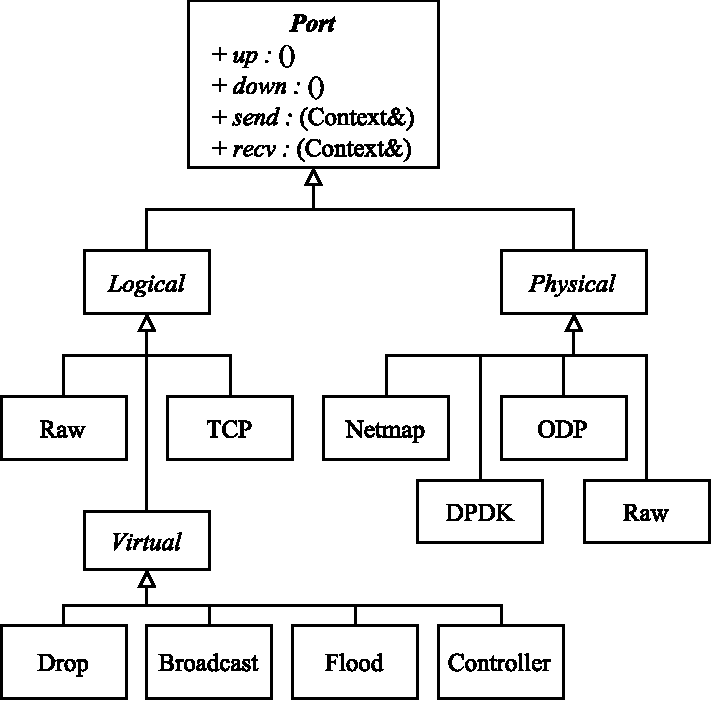
\includegraphics[scale=0.85]{ff_port_uml}
\caption{Freeflow port UML diagram.}
\label{port_uml}
\end{figure}

When packets are received by a port object, the memory that holds the raw
packet data and the context are allocated during the \emph{ingress} phase. The
underlying data store for the packet and context are owned and managed by the
port itself. Memory can be allocated from the ports internal resources (i.e.
memory mapped from a physical device address space) if present, or by the FFVM's
global buffer pool. This gives a greater amount of flexibility in that the
packet and context can exist in same memory region, potentially improving
locality. As packets leave the system during the \emph{egress} phase, this
memory is released back to the appropriate devices. Details about memory
management can be found in Section \ref{vm:memory}.

After initializing a context with a new packet, the port passes the context to
the application pipeline for processing. When the context exits the application
pipeline, the resulting action list is applied to the packet. Finally the
context enters the egress stage where the packet is forwarded to the designated
\emph{output port} set in the context, or dropped.

% The freeflow port impl lies somewhere on the spectrum...

\section{Tables}
\label{vm:tables}
In network switches, tables are used to match properties of packets
with user-defined forwarding behaviors. They can be defined using a variety of
data structures and algorithms that implement them, but generally are categorized
as \emph{exact}, \emph{prefix}, or \emph{wild card}. All three table types are
currently implemented by the FFVM, though support for prefix and wild card is
incomplete.

Each entry in a flow table contains a \emph{key} that is compared to a
certain field within the packet. Key types vary between match table types. For an
exact match table the keys are integers of a set width, defined by the
application. These keys are used to aggregate traffic containing similar
characteristics into flows. Flows can be viewed as programs, or functions,
that get executed when a packet matches their key. Each flow defines a
set of operations, or instructions, that are applied to packets. Table
\ref{flow_table} depicts a simple flow table that creates a virtual ``wire''
between two ports, where traffic received by one port is sent out the other.

\begin{table}[h]
  \centering
  \begin{tabular}{||c | c||}
   \hline
   Input Port & Flow Instruction \\ [0.5ex]
   \hline\hline
   1 & output(2); \\
   \hline
   2 & output(1); \\
   \hline
   miss & drop; \\ [1ex]
   \hline
 \end{tabular}
 \caption{A flow table that maps input ports to output ports.}
 \label{flow_table}
\end{table}

% The freeflow table impl lies somewhere on the spectrum...

\section{Instructions}
\label{vm:insn}
The FFVM hosts network applications that are dynamically loaded and executed
at run time. To avoid using an interpreter, applications must be compiled
to native shared objects. By translating the high level language down to the
target machine code, the execution of instructions provided in the binaries is
more efficient. These instructions are encapsulated in functions that can be
executed on a variety of computational devices. This allows the FFVM to take
advantage of hardware accelerators tuned for network processing.

% Freeflow insn execution lies somewhere on the spectrum...

\section{Memory}
\label{vm:memory}
Memory for raw packet data and contexts is allocated by port objects during the
ingress processing phase. The FFVM is optimized to allow for zero-copy packet
processing, where raw packet data resides in a physical device's dedicated
memory. In certain cases device packet buffers contain extra memory for user
data, which can store the context object to improve locality. Another
benefit of storing the packet and context in the same region of memory is that
the two entities can grow dynamically; the context grows as actions are appended
to it's action list and the packet grows when new protocol headers are pushed
onto a header binding environment. When a port object does not possess the
capability to provide persistent packet memory, a global packet context buffer
can be allocated by the system. Figure \ref{mem_model} illustrates the two
memory models currently supported by the FFVM.

\begin{figure}[h]
  \centering
  \begin{subfigure}[b]{0.48\textwidth}
    \centering
    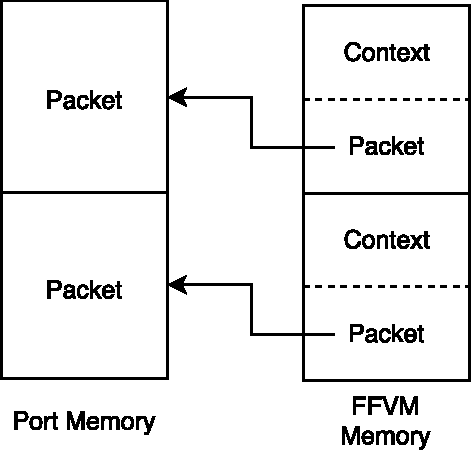
\includegraphics[scale=0.9]{mem_fig_a}
    \caption{Freeflow allocates context memory that references packet data
    in port memory.}
  \end{subfigure}
  \hfill
  \begin{subfigure}[b]{0.48\textwidth}
    \centering
    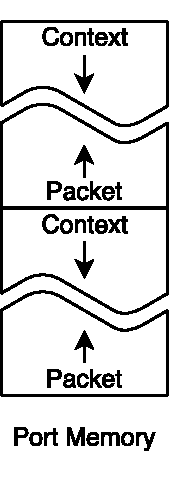
\includegraphics[scale=0.9]{mem_fig_b}
    \caption{Port memory can accommodate dynamically sized packet and context
    objects.}
  \end{subfigure}
  \caption{Freeflow packet context memory models.}
  \label{mem_model}
\end{figure}

A global buffer consists of a packet buffer, a context, and a non-zero
i.d. Packet buffers are pre-allocated 2048 byte regions that can easily
accommodate IEEE 802.3 Ethernet frames that have a maximum size of 1523 bytes.
The packet buffers are over sized to allow for the insertion of new protocol
headers that may result during or after pipeline processing. Contexts residing
in a global buffer contain a reference to the packet buffer, which by default
points to a FFVM packet buffer. The i.d. gives the offset into the global buffer
pool, and allows ports to return the i.d. back to the pool's free list. FFVM's
free list is implemented as a min-heap, providing the next available packet
buffer that can be allocated. During creation, and upon de-allocation, a packet
context buffer is set to a null state; each field in the context is default
initialized and the packet size is set to 0. In this state, referencing a
context or the packet buffer it is associated with is undefined.

% The freeflow memory model lies somewhere on the spectrum...

\section{Threading}
\label{vm:threading}
The FFVM supports multiple threading architectures to maximize execution
resource utilization. Behavior for FFVM components, such as port objects and
application pipelines, can be defined as free functions in a driver and
executed in its own thread. Threads contribute to the modular nature of the
FFVM and can be treated as building blocks to produce different execution
models. FFVM provides a simple threading interface built on the POSIX thread
library (pthread) \cite{pthread}, that executes a preallocated work routine
and passes the thread i.d. as the argument. Synchronization mechanisms and
configuration settings, or attributes, are optionally provided. The following
listing shows how a FFVM thread can be constructed with an initial i.d. and work
routine, and also re-assigned while the thread is not in a ``running'' state.

\begin{lstlisting}
void* port_work(void* arg){
  // ...
}

void* port_work2(void* arg){
  // ...
}

int main(int argc, char** argv){
  ff::Thread thread = { 1, port_work };
  thread.run();
  // ...
  thread.halt();
  thread.assign(2, port_work2);
  thread.run()
  // ...
  thread.halt();
  return 0;
}
\end{lstlisting}

In addition to the threading interface, the FFVM also provides shared data
structures such as queues and object pools. Concurrent queue implementations
exist for locked and lock-free access, allowing for more flexibility in the
threading architecture being modeled. Object pools allocate reusable global
resources that can also be shared across thread boundaries.

\section{ABI}
\label{vm:abi}
The FFVM application binary interface exposes a set of symbols and calling
conventions that can be utilized by applications at run time. These ``system
calls'' allow hosted applications to request system resources. In this section
the more pertinent functions are discussed.

\begin{lstlisting}
    ff_create_table(dp, width, n, type);
    ff_delete_table(dp, tbl);
\end{lstlisting}

A call to the \texttt{ff\_create\_table} function returns a newly allocated
flow table in the given data plane instance \emph{dp} with an application
defined key \emph{width} in bytes, an initial size of \emph{n} entries, and
matching table \emph{type}. The \texttt{ff\_delete\_table} call releases the
resources allocated in the given table \emph{tbl}.

\begin{lstlisting}
    ff_lookup_flow(tbl, k);
    ff_insert_flow(tbl, k, f);
    ff_remove_flow(tbl, k);
\end{lstlisting}

Flow entry matching is executed with a call to \texttt{ff\_lookup\_flow} which
searches for a key \emph{k} in a flow table \emph{tbl}. Table modifications can
be made using \texttt{ff\_insert\_flow} to add a new key \emph{k} with the
flow \emph{f} to table \emph{tbl}, and \texttt{ff\_remove\_flow} to remove the
key \emph{k} from the table \emph{tbl}. If the key already exists when the call
to insert is made, the associated flow object is updated, whereas a call to
remove a non-existent key from a table has no effect.

\begin{lstlisting}
    ff_output(cxt, p);
    ff_drop(cxt);
\end{lstlisting}

The \texttt{ff\_output} function sets the \emph{output\_port} field in a context
\emph{cxt} to the id of the given port \emph{p}. A call to the \texttt{ff\_drop}
function effectively sets the \emph{output\_port} field in the context \emph{cxt}
to the data plane drop port id, but terminates the further processing in the
pipeline stage it was invoked from.

\section{Conclusion}
\label{ff:concl}
Conclusion....

\chapter{EXPERIMENTS}
\label{experiments}

\section{L2 Forwarding - Wire}
\label{experiments:wire}
Emulate layer 2 forwarding of ethernet frames over TCP sockets.

\section{Threading Models}
\label{experiments:models}
Multiple...

\subsection{Single Threaded}
\label{experiments:models-single}
Server, I/O Ports, App in a single thread.

\subsection{Port Threaded}
\label{experiments:models-port}
Server, I/O Ports on seperate threads. Application shares execution
with I/O ports.

\subsection{Application Threaded}
\label{experiments:models-app}
Server, I/O Ports on a single thread. Application on a seperate thread.

\subsection{Port and Application Threaded}
\label{experiments:models-port-app}
Server, I/O Ports, and Application on seperate threads.

\section{Results}
\label{experiments:results}
Tables n stuff.

\chapter{CONCLUSIONS}
\label{concl}
SDN is still a relatively new networking architecture that is continuing
to evolve. Much of the research in this domain is experimental, searching
to establish the ``correct'' way to model basic network switch components,
host compiled network applications, and efficiently abstract networking
resources. The work presented in this thesis aims to find a balance between
high level language support and optimal hardware execution through translation
and abstraction, respectively. Contributions heavily revolve around abstracting
low level networking hardware and processing network application instructions.

The FFVM provides a concrete implementation of an abstract network switch that
provides the necessary resources required to efficiently host networking
applications. An emphasis on modularity and re-configurability allows different
virtual switches with varying capabilities, features, and resources to be
provisioned and evaluated. Low level port abstractions give users control over
networking interfaces while maintaining a high level of performance. High level
network programming languages that can be compiled down to native binary files
are able to be dynamically loaded and executed. The design and implementation
of the FFVM is a culmination of the observed requirements found necessary to
model an abstract network switch that is fully programmable, is capable of
hosting network applications, and provides access to networking hardware
resources.

\section{Future Work}
\label{concl:future}
The product of the contributions presented in this thesis is an initial
implementation of a fully programmable virtual network switch. Additional
work in this domain revolves around the two main ends of the
virtualization-materialization spectrum: improved hosting support for more
high level network programming languages and optimizations to hardware resource
usage.

With respect to high level languages, support for the POF programming language
would be easier as their models for decoding packet protocol header fields and
forwarding behavior align with the FFVM context binding environment and flow
table constructs. Other well established networking programming languages,
such as P4, could also be considered to improve portability and application
hosting capabilities.

Low level hardware abstraction aligns with the problems found in the domain of
heterogeneous computing. Advances in that field can provide insight into future
design and implementation strategies that could be incorporated into the FFVM.
The usage of an IR allows for machine specific intrinsics to optimize the code
generated by compilers to take full advantage of all computing resources
available on a target system.

% \subsection{OVS Integration}
% \label{future:ovs}
% How we can distribute FF apps using OVS.

% \begin{figure}
% \centering
% 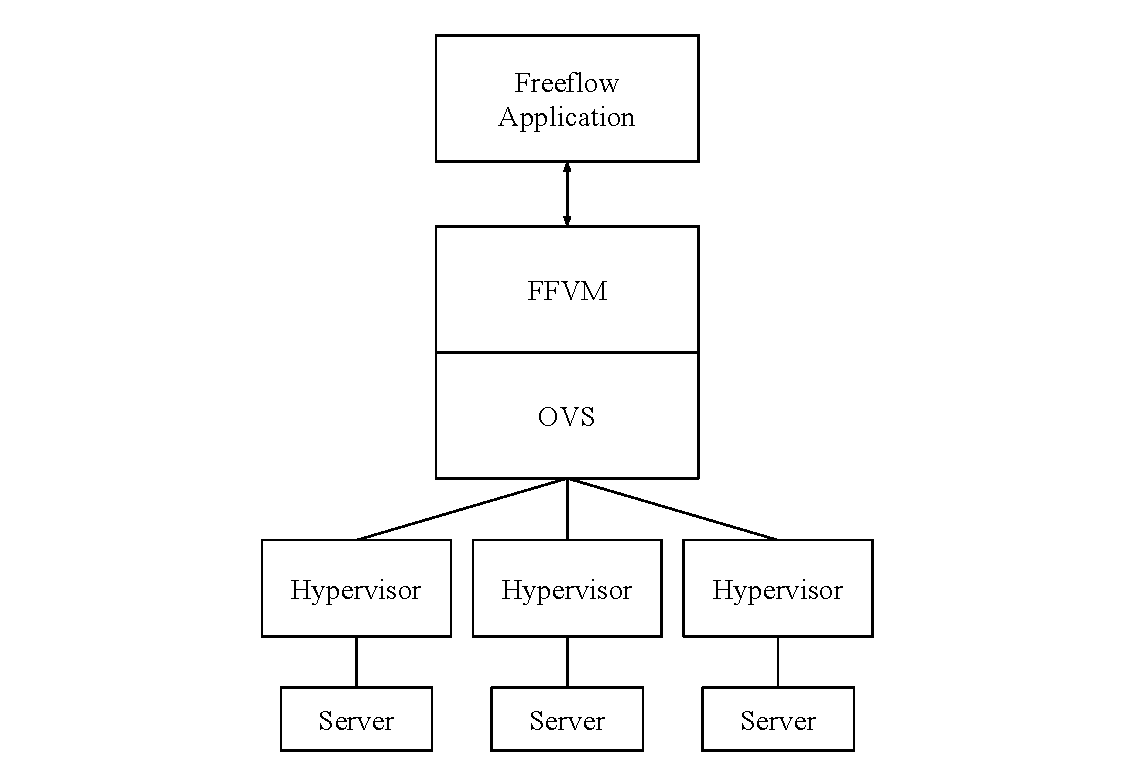
\includegraphics[scale=0.5]{ff_ovs_arch}
% \caption{Freeflow running ontop of OVS.}
% \label{ff_ovs_arch}
% \end{figure}

\bibliographystyle{unsrt}
\bibliography{bio}
%If you have n appendices, then use the \appendices{n} command below
%followed by n \input{filename} commands, similar to the \input{chapx}
%commands above.
% DO NOT USE SECTIONS OR SUBSECTIONS IN AN APPENDIX OR APPENDICES
\appendix{1}
\chapter{APPENDIX TITLE GOES HERE}
\label{appendix}

\section{First Section}


\section{Second Section}


\subsection{First Subsection}


\section{Third Section}

\end{document}
